\chapter{Asking Texans Their Best Life Advice (Dallas)}

This School of Hard Knocks interview, prepared here as a companion chapter by LazyingArt LLC through Video2Book, is not a blackboard lecture. Even so, it has a real analytic spine. We are taken through a sequence of live encounters in downtown Dallas, and the same question is asked again and again: what career choices, financial decisions, and operating habits actually mattered? The mathematics is therefore modest and editorial rather than original to a board, but the mechanisms are recognizable. Debt can be extinguished or carried. Assets can appreciate or be missed. Effort can be turned into productive capacity. Low fixed obligations can buy optionality. The lecture moves by these mechanisms, one witness at a time.

\section{Dallas as a Field Laboratory}

We begin with scene-setting rather than doctrine. James frames the episode as a second Dallas outing and fixes the governing theme before any interview begins: we are asking people for the best financial decision they have made, and we are asking what kind of work, judgment, and discipline stood behind it.

That opening matters. It tells us how to read everything that follows. We are not looking for one master formula. We are watching a field experiment in which the same prompt is put to different lives. The order is important: first the city, then the question, then the testimonies.

\section{Career Formation, Effort, and Debt Discipline}

The first respondent gives us the lecture's earliest structural point. A career path need not be straight to be economically real. The speaker begins in psychology, moves through management and information systems, and ends as an owner of four companies. The lesson is not that credentials are irrelevant; it is that credentials by themselves are not the whole story. The interview immediately compresses that thought into a directional rule: if we want the business-owner upside, we must put in business-owner time.

A minimal way to record that claim is
\begin{equation}
I \uparrow \Longrightarrow R \uparrow,
\end{equation}
where \(I\) denotes time and effort committed, and \(R\) denotes the results one can plausibly extract. This is not a theorem, and the lecture gives us no calibrated map from input to output. It is only a directional statement: the fantasy of owner-level return with casual \(9\)-to-\(5\) effort is rejected at once.

The interview then pivots, very quickly, from effort to household finance. The first concrete financial decision is to pay off credit-card debt and not rebuild it. We can write the bookkeeping identity in a compact weekly form. Let \(D_{\mathrm{cc}}^{(n)}\) be revolving credit-card debt at the start of week \(n\), let \(c_n\) be new charges during that week, and let \(p_n\) be the payment made at settlement. Then
\begin{align}
D_{\mathrm{cc}}^{(n+1)} &= D_{\mathrm{cc}}^{(n)} + c_n - p_n, \\
p_n &= D_{\mathrm{cc}}^{(n)} + c_n
\quad \Longrightarrow \quad
D_{\mathrm{cc}}^{(n+1)} = 0.
\end{align}

\paragraph{Worked update rule.}
The speaker's practical rule is exactly the disciplined choice in the second line. We charge during the week, but at settlement we pay the entire carried balance plus the week's new charges. The update then returns us to zero carried debt. There is no need here for an interest-rate calculation; the point of the interview is more primitive and more decisive. The target state is
\begin{equation}
D_{\mathrm{cc}}(t_{\mathrm{settlement}})=0.
\end{equation}

The same respondent then sharpens the rule by introducing a cash test for extravagant consumption. For a contemplated purchase \(x\) of price \(P_x\), with available cash \(C\), the advice becomes
\begin{equation}
C \ge P_x \Rightarrow \text{buy }x,
\qquad
C < P_x \Rightarrow \text{do not buy }x.
\end{equation}
Again, this is not a universal law of finance. It is a guardrail. The lecture is telling us that before we speak about leverage, investing, or entrepreneurship, we must first know whether we are using debt as a tool or letting it become a habit.

\section{Technology, Social Skill, and the First Asset Example}

The next movement turns from debt to employability. The speaker in technology says two things at once. First, entry is easier now because information is available online. Second, the easier access does not remove the need to like the work well enough that it ceases to feel merely like work. We are given a labor-market correction: technical access is not the same thing as vocation.

That correction becomes sharper in the hiring remark that follows: technology is not a social skill. In other words, the lecture does not let us reduce market value to credential plus tool familiarity. One still has to function among other human beings. This matters because the whole interview is building toward a wider notion of capital. Skill matters, but so do presentation, interaction, and judgment.

The section closes with the first explicit numerical example in the lecture: a house purchase that, according to the speaker, has appreciated by about two hundred thousand dollars. If \(V_h(t_0)\) denotes the house value at purchase and \(V_h(t_1)\) the later value, then the reported appreciation is
\begin{equation}
\Delta V_h = V_h(t_1)-V_h(t_0) \approx \text{\$200{,}000}.
\end{equation}

\begin{remark}
This is an anecdotal appreciation statement, not a general housing theorem. The lecture gives us no purchase price, leverage, maintenance cost, tax burden, or holding interval. What it does give us is the mechanism the speaker cares about: ownership can convert a rise in asset value into captured household equity, whereas rent does not.
\end{remark}

We may therefore summarize the first part of the lecture this way. The path begins with effort, tightens into debt discipline, broadens into employability, and then yields its first asset-side illustration in owner-occupied housing.

\section{Risk, Drift, and the Million-Dollar Stress Test}

The next witness is a counselor, and the lecture changes register. We are no longer speaking only about discipline and asset capture. We are speaking about what kind of person can even move through the world well. The counselor's most rewarding experience is watching students grow from eighth graders into adults. That naturally leads to advice for people just entering the real world.

What appears first is a verbal stumble and then a correction. The speech begins as though caution were the message, but it immediately turns: do not be afraid to take a risk. This turn should be preserved. The lecture is not advocating chaos. It is exposing the danger of a life that never leaves the safe corridor.

\subsection{Question \& Answer}

\paragraph{Question.}
Is the safe path actually safe?

\paragraph{Answer.}
Not if safety means permanent avoidance of initiative. The lecture's stress test makes this plain. James asks what one would do if one had to make a million dollars in a year and life depended on it. The answer is comic and desperate at once: there is no plan, only the fantasy of a robbery. That is the point. A life organized around avoiding risk can arrive at a moment of pressure with no constructive path at all. The right correction is not recklessness. It is the cultivation of agency before the emergency arrives.

This is why the counselor's section belongs exactly here. The lecture needs a local tension before it moves on. The earlier advice taught us how not to get trapped by debt. This section asks whether we can also avoid getting trapped by timidity.

The practical aftershock comes immediately in the financial advice to college students: do not take loans and do not open credit cards lightly. So the lecture does not abandon prudence after its defense of risk. Rather, it holds the two ideas together: do not be financially careless, but do not build a whole life on passivity.

\section{Self-Investment, College Skepticism, and Intentionality}

The Spider-Man segment is a hinge, not a novelty. The odd-jobs answer is humorous, but the financial advice that follows is serious and structurally important. The best decision, the speaker says, was investing in oneself. The money that had gone into things that ``wasn't it'' should instead go into the person, the tools, and the equipment that make future work possible.

A compact way to represent the claim is
\begin{equation}
K_{\text{self}} = K_{\text{skills}} + K_{\text{tools}} + K_{\text{equipment}}.
\end{equation}
Here \(K_{\text{self}}\) is not a measured stock in the transcript; it is a clean way to record the mechanism. We invest first in productive capacity, and only then do we expect better economic outcomes.

The next question is whether college is necessary. The answer is no, but the important thing is why. The speaker does not merely reject school in the abstract. He says that the ordinary school path often sorts people into preset roles. If we want to make our own way and leave a legacy, then we must know what we want and build toward it. The lecture is therefore moving from a polemic against credentialism to a constructive doctrine of intention.

That constructive doctrine is made explicit in the advice to the younger self. If we are clear about what we want to accomplish, we are more likely to arrange the steps that bring it about. If we remain ``flippy floppy,'' the path itself becomes flippy floppy. In compact form,
\begin{equation}
G \text{ clear}
\Longrightarrow
\Pr(\text{goal attainment}) \uparrow.
\end{equation}

\begin{remark}
This probability arrow is heuristic. The lecture offers no data and no formal decision theory. What it offers is a strong qualitative claim: clarity of aim reorganizes conduct.
\end{remark}

So the order here is essential. We begin with self-investment, we pass through skepticism about formal credentials, and we arrive at intentionality. The lecture is no longer only about how to spend less badly. It is about how to become a person whose expenditures, tools, and daily actions point in one direction.

\section{Household Architecture: Partner, Family, and Work Ethic}

The next move is one of the most important in the chapter. The lecture broadens the category of a financial decision until it includes the architecture of a life. One speaker says the best decision was marrying someone with a good financial mind, or more fully, finding a partner with similar aspirations and goals and then working together toward them over time. The financial mechanism here is not a spreadsheet entry. It is alignment.

We should say this carefully. The lecture is not offering a return-on-investment theorem for marriage. It is saying that a household can either concentrate effort or dissipate it. Shared direction matters economically because it stabilizes long-run action.

A related expansion appears in the public servant's answer: the best investment was investment in the family. The daughters are the ``bombs,'' the parents ``did the right thing,'' and the family is treated as the true object of investment. Once again, finance is being widened beyond budgeting into intergenerational design.

At exactly this point, another speaker rejects the idea that a college degree is necessary for success and substitutes trade plus work ethic. This belongs here, not earlier, because the lecture is now looking at the whole structure of a life: partner, family, skill, labor, and the ethos of work.

\begin{definition}
In the language of this lecture, a financial decision is any durable choice that shapes future cash flow, future capacity, future alignment, or future opportunity.
\end{definition}

That definition is editorial, but it names what the transcript is plainly doing. The lecture has moved from balances and purchases to households and trajectories.

\begin{table}
\begin{center}
\begin{tabular}{|l|l|l|}
\hline
Decision type & Representative claim & Main mechanism \\
\hline
Pay off cards & Stop carrying revolving debt & Release cash-flow pressure \\
Cash test & Do not finance extravagance & Block bad liability growth \\
Buy a house & Ownership captured appreciation & Convert price rise into equity \\
Invest in self & Buy tools and build skill & Raise productive capacity \\
Choose partner well & Align aspirations and conduct & Stabilize long-run action \\
Invest in family & Treat household as the project & Build intergenerational strength \\
Learn a trade & Outwork the credential signal & Convert effort into income \\
Relocate & Move where opportunity is thicker & Expand the accessible option set \\
Stay low debt & Preserve mobility & Increase optionality \\
Be original & Differentiate the work & Increase market response \\
\hline
\end{tabular}
\end{center}
\end{table}

\section{Geography, Optionality, and Creative Differentiation}

The law-enforcement speaker adds another layer. The best financial decision was moving to Dallas from Mississippi and, just as importantly, not spending money on nonsense after the move. This is the lecture's clearest statement that geography is itself a financial variable. The move is not presented as aesthetic preference; it is presented as a shift in the density of available opportunity.

A compact editorial shorthand for that claim is
\begin{equation}
A(\text{Dallas}) > A(\text{Mississippi}),
\end{equation}
where \(A(L)\) denotes the opportunity set accessible at location \(L\).

\begin{remark}
This inequality records the speaker's judgment, not a measured statistic. It is useful because it names the lecture's mechanism: the same person, with the same labor, may face a different opportunity frontier in a different place.
\end{remark}

The next respondent then turns this idea into a more abstract rule. The best financial decision was paying off debts, not because debt is always bad in principle, but because staying low debt and high income preserves the ability to move, travel, and jump when an opportunity appears. This is one of the cleanest mechanisms in the lecture:
\begin{equation}
D \downarrow,\qquad Y \uparrow
\qquad \Longrightarrow \qquad
O \uparrow,
\end{equation}
where \(D\) is debt burden, \(Y\) is income flow, and \(O\) is optionality.

\begin{definition}
Optionality means the practical freedom to move, invest, travel, or change plans when an opportunity presents itself, without first spending months unwinding obligations.
\end{definition}

The final major witness is in music. Here the lecture folds practice, collaboration, and creativity into the same analytic frame. The advice is to practice, to work with others, and not to be afraid of one's creativity because the originality is what people are looking for. A compact way to record the claim is
\begin{equation}
O_r \uparrow \Longrightarrow R_{\text{market}} \uparrow,
\end{equation}
where \(O_r\) denotes originality and \(R_{\text{market}}\) denotes market response.

We should again be cautious. This is not a law of demand. It is a practical heuristic from a creative worker: when everything is easy to copy, differentiation matters.

Because the lecture gives us no board diagram, we may summarize its implicit architecture with a small editorial schematic:

\begin{figure}
\begin{center}
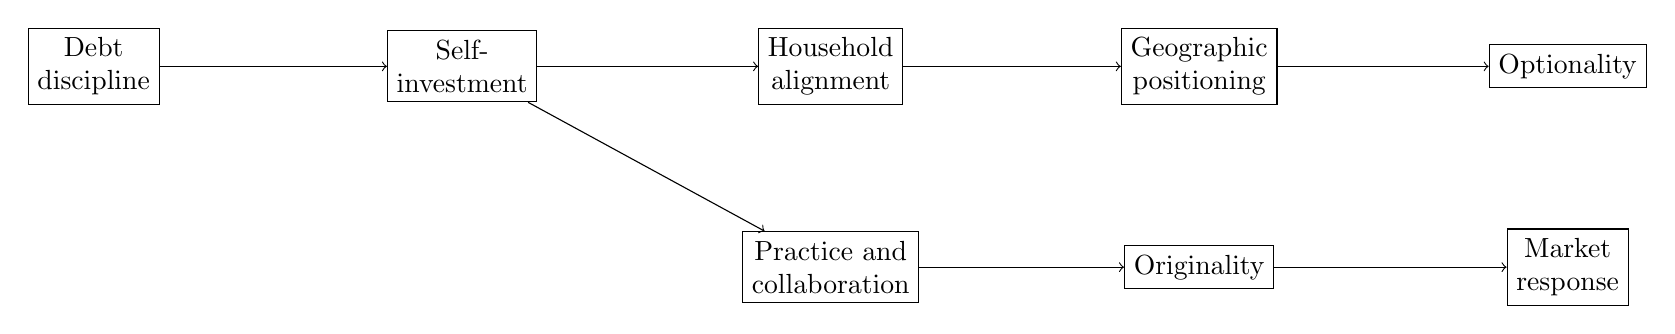
\begin{tikzpicture}[x=2.6cm,y=1.7cm]
\node[draw, rectangle, align=center] (a) at (0,0) {Debt\\discipline};
\node[draw, rectangle, align=center] (b) at (1.8,0) {Self-\\investment};
\node[draw, rectangle, align=center] (c) at (3.6,0) {Household\\alignment};
\node[draw, rectangle, align=center] (d) at (5.4,0) {Geographic\\positioning};
\node[draw, rectangle, align=center] (e) at (7.2,0) {Optionality};

\node[draw, rectangle, align=center] (f) at (3.6,-1.5) {Practice and\\collaboration};
\node[draw, rectangle, align=center] (g) at (5.4,-1.5) {Originality};
\node[draw, rectangle, align=center] (h) at (7.2,-1.5) {Market\\response};

\draw[->] (a) -- (b);
\draw[->] (b) -- (c);
\draw[->] (c) -- (d);
\draw[->] (d) -- (e);

\draw[->] (b) -- (f);
\draw[->] (f) -- (g);
\draw[->] (g) -- (h);
\end{tikzpicture}
\end{center}
\end{figure}

This figure is not a recovered lecture image. It is an editorial map of what the interviews cumulatively build: discipline, then capacity, then alignment, then positioning, and finally the ability either to seize opportunities or to create differentiated work.

\section{Summary}

The Dallas episode begins as a street interview and ends as a compact theory of practical capital. We start with hard work, debt repayment, and the refusal of extravagant borrowing. We then add employability, social skill, risk tolerance, and self-investment. After that the frame widens further to include intentionality, partner choice, family life, work ethic, relocation, mobility, and originality.

What makes the lecture worth preserving is precisely this widening. A financial decision is not treated as a narrow accounting event. It is treated as a durable choice about liabilities, assets, skills, households, locations, and the kind of work one intends to do. The chapter therefore closes where the interview closes: not with a theorem, but with a family of mechanisms. Reduce the liabilities that trap us. Build the capacities that compound. Align the life. Move where the game is live. Keep enough freedom to act when the opening comes.